\chapter{Related Work}
\label{related}
In this chapter, several related research papers are explained that provide solutions to distribute computations for parallel execution. The first section covers OpenCL based approaches for parallelizing workloads on a single machine. The second section exhibits cluster distribution approaches based on OpenCL and CUDA.

\section{OpenCL Single Machine Distribution}

\subsection*{SOCL}
SOCL is an OpenCL based framework by \citeauthor{socl} that offers the following key features\cite{socl}:
\begin{itemize}
    \item Scheduling and load balancing of OpenCL kernels across multiple devices
    \item Management of memory transfers and coherency
    \item Dynamic adaption of kernel granularity
\end{itemize}

SOCL acts as a middleware with its own OpenCL ICD utilizing other installed ICDs on a machine. Thus, it is able to implement functionalities such as shared command queues for multiple devices by hiding the divided command queues of each device behind its API. Through this method load balancing techniques can also be applied.

One of the main features is the automatic granularity adaption of kernels, which allows the appropriate partitioning of tasks according to respective performance capabilities of devices in a heterogeneous cluster. To enable the adaption, programmers have to supply the framework with a function that indicates how to divide the kernel with its corresponding data.

\subsection*{Static multi-device load balancing for OpenCL}
\citeauthor{delalama_2012} published an approach for executing a single kernel on multiple devices as well as a load balancing mechanism based on each device's computing capabilities\cite{delalama_2012}.
Instead of splitting the data into smaller parts, they replicate its entirety across the utilized devices and merge the resulting output buffers. The merge process is based on an algorithm that finds buffer elements that underwent write operations during the execution and therefore should be present in the final result.


\subsection*{STEPOCL}

\citeauthor{stepocl} present a framework called STEPOCL, which offers programming multi-device applications using a specifically developed domain specific language\cite{stepocl}. Their promoted features are linear performance scaling with increasing device count as well as comparable performance to manually written OpenCL applications.

For a successful distribution of a kernel across multiple devices STEPOCL requires OpenCL kernels to be submitted with an accompanying configuration that provides the following information:
\begin{itemize}
    \item The data layout, which is used to split the data into subdivisions.
    \item A tiling configuration depending on the targeted device types. E.g. specific work-group sizes for CPUs and GPUs.
    \item A meta control flow of the application, which for example allows iterative algorithms.
\end{itemize}

Utilizing the configuration, an OpenCL kernel is transformed to a new OpenCL kernel that supports computing the partitioned data. During this compilation step STEPOCL identifies available devices that it can distribute the submitted workloads to. The distribution ratio of workloads per device is determined dynamically through a profiling mechanism that takes into account the performance of each device during the previous iteration of a kernel execution. Therefore it is especially meaningful for iterative algorithms, such as n-body or k-means.

\subsection*{Fluidic Kernels}

The paper by \citeauthor{fluidic} proposes parallelizing kernels among the CPU and GPU of a machine\cite{fluidic}. They showcase two workloads that benefit either from CPU or GPU. In order to execute a kernel in parallel on both devices, it is launched on the CPU as well as the GPU. While the GPU processes the submitted work-groups from the front, the CPU starts execution from the other end in so-called subkernels. After each finished subkernel, the CPU reports to the GPU the current work-group ID. During execution of each group, the GPU checks whether the current work-group has been processed yet and can therefore identify when it has reached work-groups that have already been computed by the CPU. Due to this mechanism, the overall task is distributed according to the computational capabilities of the participating devices.


\section{OpenCL and CUDA Cluster Distribution}
\label{cluster_distribution}
\subsection*{dOpenCL}

dOpenCL wraps the local OpenCL implementation in its own provided ICD. When the driver is used on the host, it forwards the API calls to specified machines in the network, which run a dOpenCL daemon\cite{dopencl}. The calls are received by the daemon and executed using the available OpenCL installation on the remote machine with the results being returned via network. This allows utilizing remote devices as if they were installed locally in the host machine. For example, a remote GPU would appear as if it was installed in the local machine's peripheral component interconnect express (abbr. PCIe) slot. Therefore OpenCL kernels do not require changes to run remotely as dOpenCL hides network transfers behind the standard OpenCL API. An overview of the architecture for an example cluster is shown in figure \ref{img:dopencl_arch}.

\begin{figure}[H]

	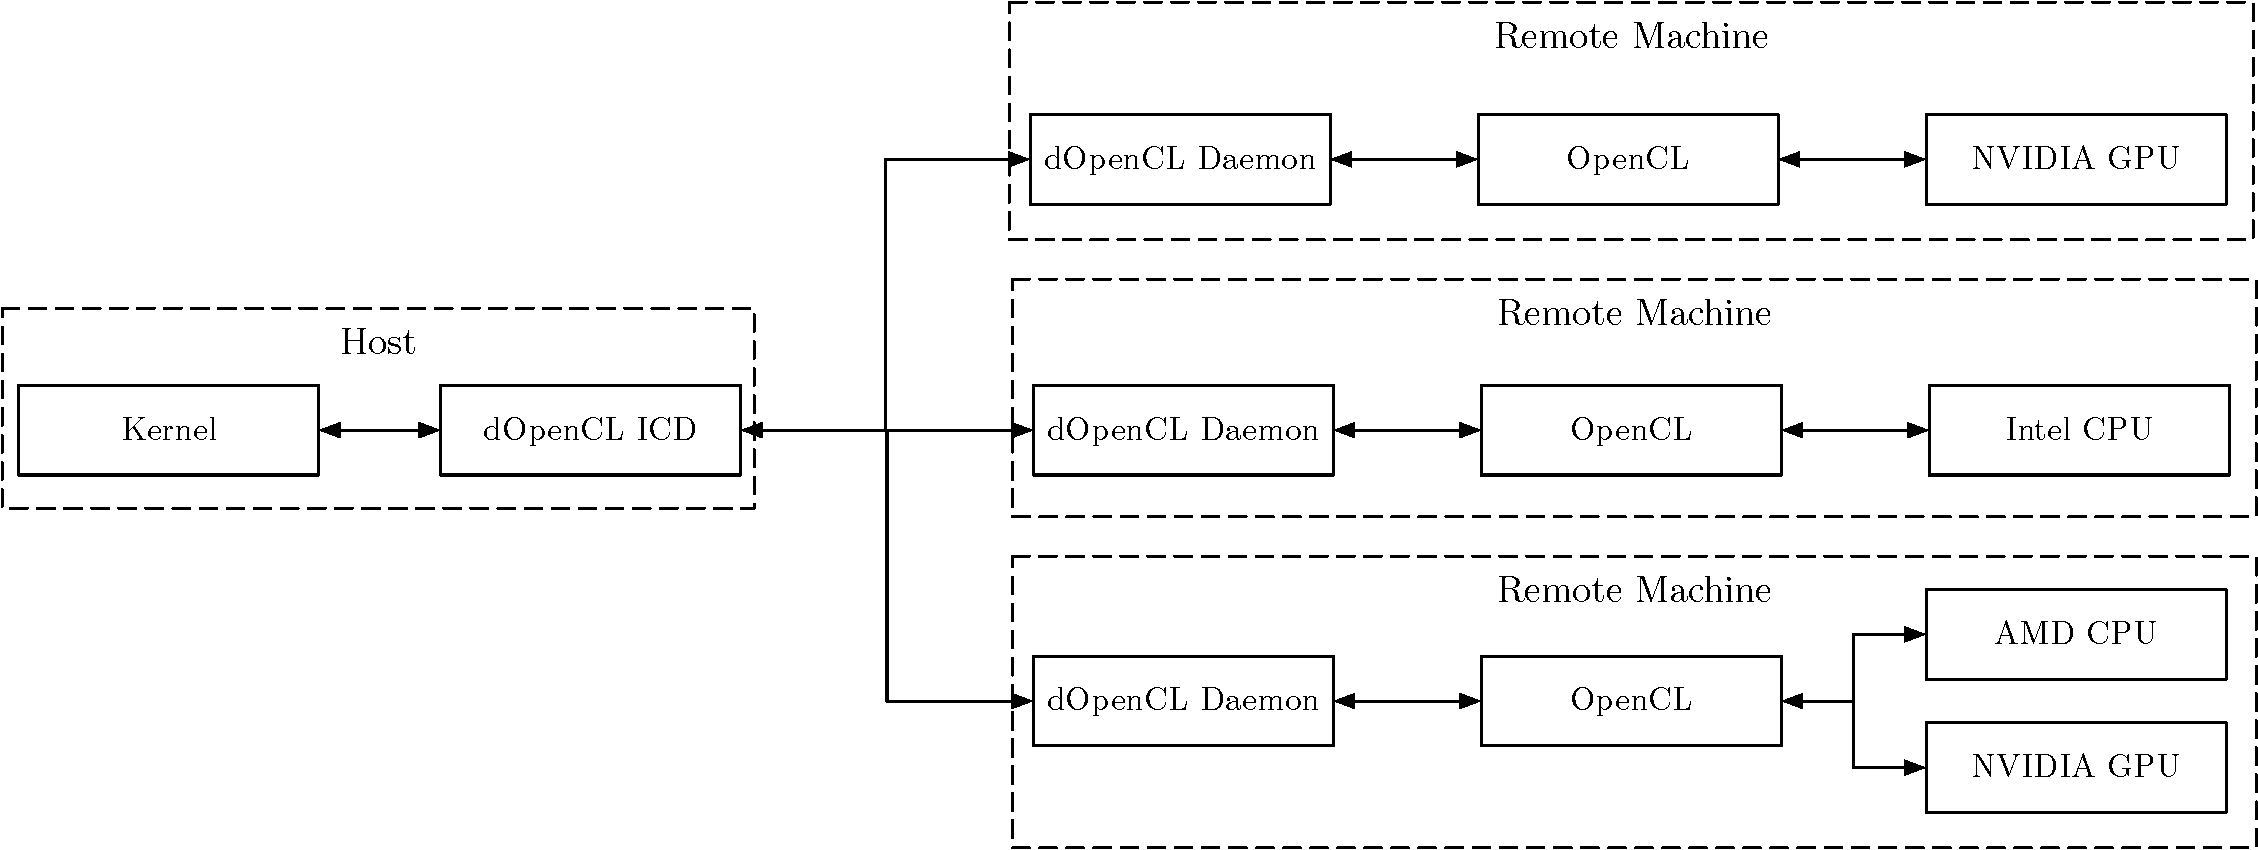
\includegraphics[width=0.95\textwidth]{drawings/dopencl_arch.pdf}
	\centering
	\caption{dOpenCL Architecture Overview}
	\label{img:dopencl_arch}
\end{figure}

dOpenCL supports shared cluster environments, in which multiple OpenCL programs run concurrently, by employing a device manager. It processes the assignment of devices to specific kernels and keeps track of device utilization within the cluster. Thus, it ensures that a device is used only by a single kernel at each point in time.

In their evaluation, \citeauthor{dopencl} show that for workloads with small datasets dOpenCL performs and scales well. They also compare dOpenCL's ability to transfer data to and from remote devices using Gigabit Ethernet against PCIe bandwidths. In the results, they conclude that dOpenCL reads the data 4.5x slower and writes 50x slower than their measured PCIe connection.

\subsection*{VirtualCL}

Similarly to dOpenCL, VirtualCL forwards OpenCL API calls to remote machines within a cluster\cite{virtualcl}. It wraps its own ICD around the calls and refers them to running daemons on the remote machines. \citeauthor{virtualcl} evaluate various applications comparing the local versus remote runtimes via VirtualCL. They show that network bandwidth and latency are the main bottlenecks of their solution but that long and compute intense kernels with low data transfers perform well.

VirtualCL offers an extension, called SuperCL, which is aimed at reducing network transfers by allowing multiple kernels being submitted to a remote node for serial execution. When these kernels depend on each other, the results are not transferred back and forth but stored in temporary buffers. It also supports more complex use cases like alternating iterative kernels on the same data set.

\subsection*{SnuCL}

SnuCL represents another library, aside from dOpenCL and VirtualCL, that provides a mechanism to access compute devices of a cluster as if they were installed in a single local machine\cite{snucl}. Instead of simply forwarding API calls to remote machines, SnuCL heavily transforms kernels depending on the available runtimes of a machine. For example, it translates OpenCL to CUDA when only the CUDA platform is provided by the machine. Additionally, it can transform OpenCL code to C, which is then executed within a thread for each core of a CPU.

Furthermore, SnuCL introduces a virtual global memory, in which buffers may be shared among devices. It manages the consistency among shared buffers and attempts to minimize copy operations throughout the execution in order to save bandwidth. This is achieved by translating the OpenCL code to C, which is then used to identify whether a buffer will be written during execution. Buffers that are not written can therefore remain on a device without the requirement to be copied back to the host.

\subsection*{DistCL}
DistCL aims at merging multiple GPUs as a single virtual OpenCL device\cite{distcl}. To achieve this, it abstracts the devices by representing them as one unified device while handling kernel distribution and data transfers transparently. In order to enable parallelization of a kernel, DistCL automatically splits it into multiple kernels with their respective required data, called subranges. For this, programmers have to supply a meta-function that determines the memory access pattern. Based on the given function, DistCL can transfer only relevant data to a device that executes a subrange.

\subsection*{MultiCL}

MultiCL is built on top of SnuCL and promises to schedule kernels appropriately among multiple heterogeneous devices in a cluster\cite{multicl}. It offers a round robin approach as well as an autofit mechanism. When queuing a kernel, a flag can be attached to it, which labels the assumed execution type. The available flags comprise \textit{compute intense}, \textit{memory bound}, \textit{I/O bound} or \textit{iterative}.

The scheduling mechanism is able to employ a static or a dynamic algorithm. In their static scheduling approach, they profile all available devices in regards to memory bandwidth and instruction throughput. Based on these measurements, the best fitting device is selected with respect to the kernel flag. In their dynamic scheduling algorithm they apply different mechanisms depending on the flag:

\begin{description}[align=left,leftmargin=0cm]
\item [Iterative] Cache previous kernel execution times to find best performing device
\item [Compute-intensive] Kernels are transformed to smaller minikernels that are profiled on every available device to receive a performance indicator
\item [I/O-intensive] Extended data caching and minimized transfer operations for distributed executions
\end{description}

\subsection*{rCUDA}

rCUDA aims to reduce the number of GPU accelerators in a cluster by sharing the accelerators across machines within the network\cite{rcuda}. Thus, not every machine is required to have a GPU installed. The applied technique comprises API forwarding to execute CUDA commands on the remote server and retrieve the respective result.

The main focus of the presented evaluation lies on power savings. When reducing the number of accelerators in a considered cluster by 90\%, a 20\% decrease in power consumption could be determined. Still, the authors are aware that this reduction can lead to a significant performance degradation depending on the application requirements within the cluster.

\subsection*{Virtualizing CUDA Enabled GPGPUs on ARM Clusters}

\citeauthor{arm_virtual_cuda} present an architecture in which a cluster of low-powered ARM devices accesses powerful remote NVIDIA GPUs through a virtual interface\cite{arm_virtual_cuda}. Their approach is based on API forwarding but features the connection of a private cluster to machines that are located at a cloud provider. In their example cluster, they connect local ARM devices to GPUs that are provided by Amazon's cloud.
